\section{Tracking Defenses}
\label{sec:tracking-mitigations}


%%
\begin{figure*}[tp]
    \centering
    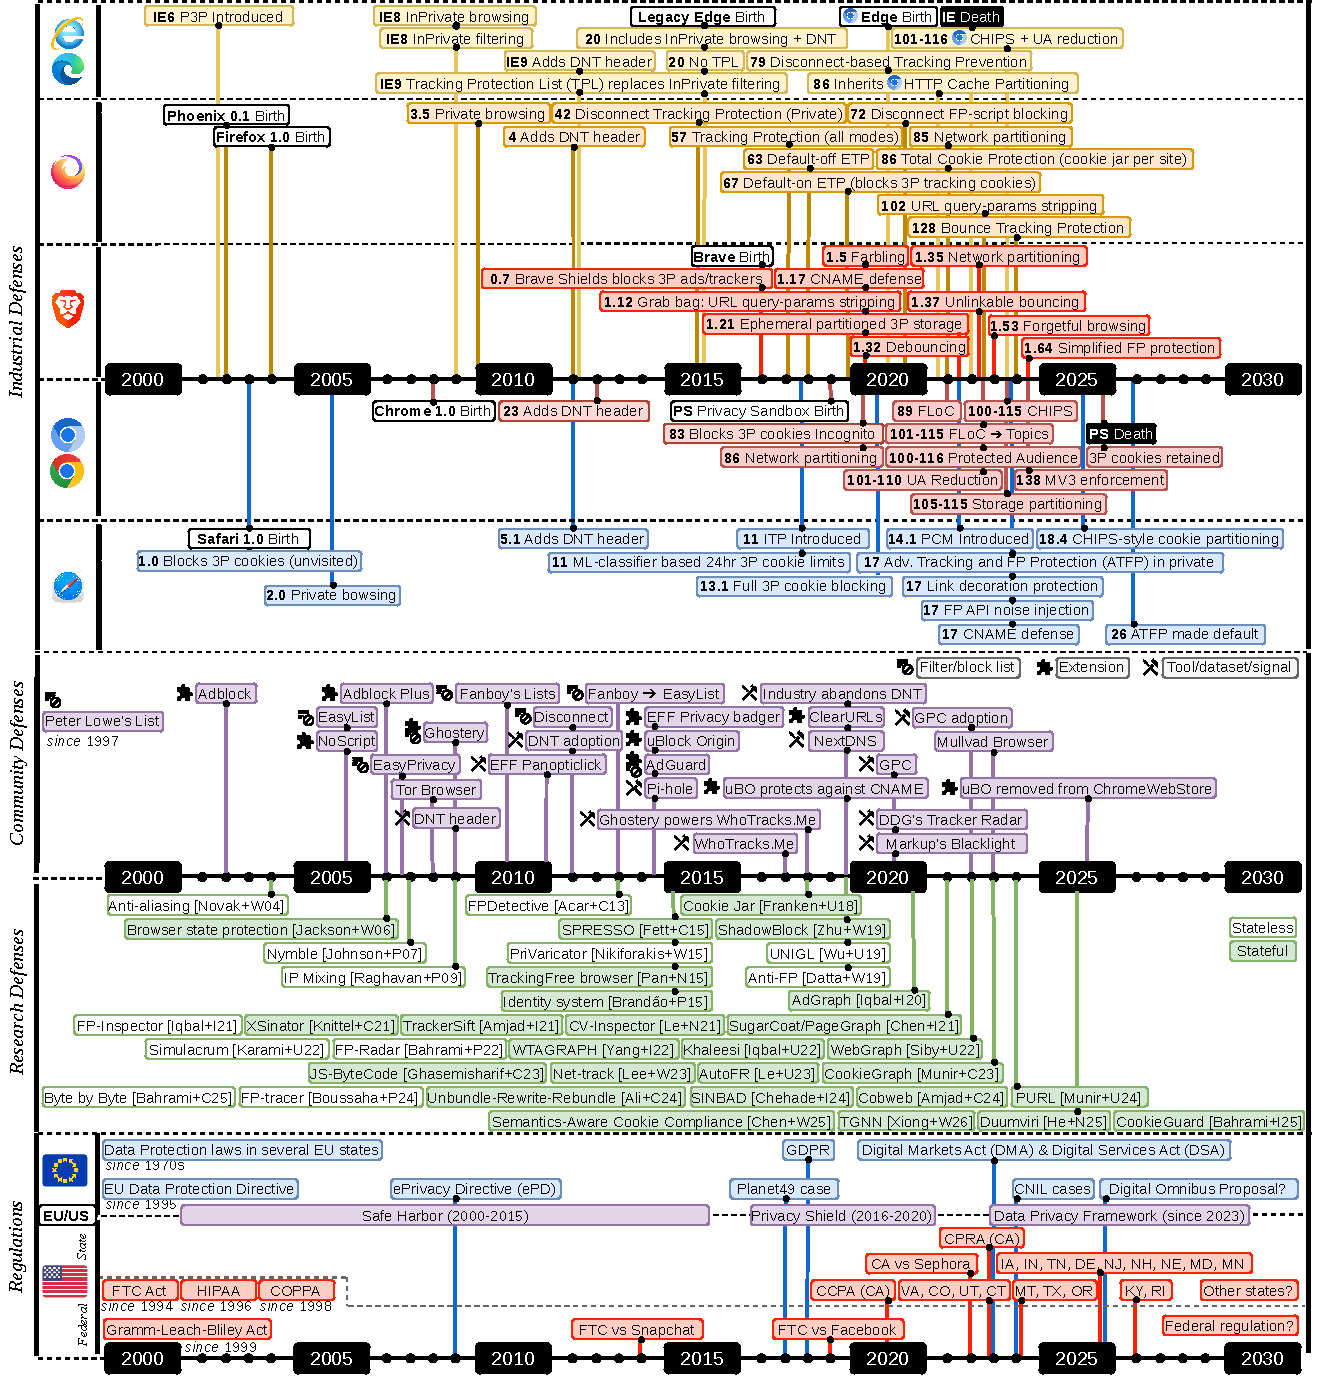
\includegraphics[width=\textwidth]{figures/evolution-tracking-defenses-regulations.pdf}
    \caption{Evolution of \emph{industry-based}, \emph{community-based}, and \emph{research-based} web tracking defenses from 2000--2026 with EU and US regulations overview.}
    \label{fig:evolution-defenses}
\end{figure*}


%%
We systematize tracking defenses across three dimensions in accordance with the criteria defined in \autoref{tab:systematization-criteria}: \textit{industry-based}, \textit{research-based}, and \textit{community-based}.
%
Following the methodology described in \autoref{sec:methodology}, we first curate industry-based and community-based defenses as described under \autoref{sec:systematization} (see \autoref{tab:defenses-industrial} for industry-based defenses and \autoref{tab:defenses-community} for community-based defenses) and research literature comprising 58 papers on tracking defenses as obtained in \autoref{sec:lit-review} (see \autoref{tab:defense-mechanisms}).
%
Each defense technique is grouped by its goal either as \colorbox{cellred}{detection \& blocking} or \colorbox{cellyellow}{signal reduction \& obfuscation}. 
%
For industry-based and community-based defenses, we identify 12 defense techniques against stateful tracking (see \autoref{tab:stateful-tracking-defenses}) and 11 defense techniques against stateless tracking (see \autoref{tab:stateful-tracking-defenses}). 
%
We also systematize support of each defense technique across each browser (Edge, Firefox, Brave, Chrome, and Safari). 
%
For research-based defenses, we identify 8 defense techniques described in \autoref{tab:defense-goal-mechanism-taxonomy}, grouped by the two aforementioned goals. 
%
The mapping of each defense paper to these defense techniques is represented in \autoref{tab:defense-mechanisms}.
%
Each defense technique across the three dimensions is also systematized based on artifact the defense is applied to and its deployment. 


%%
We organize this section similar to \autoref{sec:tracking-techniques}, by tracked state: defenses against \textit{stateful} tracking (\autoref{sec:stateful-defenses}), \textit{stateless} tracking (\autoref{sec:stateless-defenses}), and \textit{mixed} tracking (\autoref{sec:mixed-defenses}).
%
Within each, based on who develops the defense, we systematize them under industry-, research-, and community-based defenses. 
%
\autoref{fig:evolution-defenses} plots the evolution of tracking defenses along each of these three dimensions as a single timeline from 2000 to 2026. 


%%
\subsection{Defenses Against Stateful Tracking}
\label{sec:stateful-defenses}


%%
\begin{table*}[t]
  \scriptsize
\centering
\caption{\textbf{Industrial and community defenses against stateful tracking} across two defense goals: \colorbox{cellred}{detection \& blocking} and \colorbox{cellyellow}{signal reduction \& obfuscation}. Protects against: \iconCookie: Cookie-based tracking, \iconURL: Navigational tracking, \iconFingerprint: Fingerprinting, \iconJS: JavaScript-based tracking, \iconSC: Side-channels. ``(D)'' is by-default, ``(P)'' is private-mode only, and ``(O)'' is opt-in based.}
\label{tab:stateful-tracking-defenses}
\footnotesize
\renewcommand{\arraystretch}{1.1}
\scalebox{0.74}{%
\begin{tabular}{
  m{3.15cm}
  m{3.0cm}
  m{3.0cm}
  m{3.0cm}
  m{3.0cm}
  m{3.0cm}
  m{3.0cm}
}
\toprule
\textbf{Defense Technique}\newline (\textbf{Protects Against}) & \textbf{Brave} & \textbf{Chrome} & \textbf{Edge} & \textbf{Firefox} & \textbf{Safari} & \textbf{Community Defense} \\
\toprule

\cellcolor{cellred} Blocking\newline3P cookies/storage\newline\newline \iconCookie
  & all 3P cookies and storage blocked via Shields (D)
  & 3P cookies and storage blocked in Incognito (P)
  & known tracker 3P cookies blocked (D)
  & known tracker 3P cookies blocked in ETP stnd. (D);\newline all 3P cookies blocked in ETP Strict (D)
  & all 3P cookies and storage blocked (D)
  & Tor blocks 3P cookies and storage\newline uBO, Privacy Badger, AdGuard, Ghostery blocks known tracker cookies via filter lists \\
\midrule

\cellcolor{cellyellow} Partitioning\newline3P cookies/storage\newline\newline \iconCookie\,\iconSC
  & uses Chromium's storage partitioning;\newline ephemeral 3P cookies/storage cleared on tab close (D)
  & opt-in partitioned cookies via \texttt{Partitioned} attribute: CHIPS;\newline storage partitioned by top-level site (D)
  & uses Chromium's CHIPS and its storage partitioning (D)
  & Total Cookie Protection: separate cookie jar per top-level site for all embedded 3P origins;\newline all storage APIs isolated per top-level site (D)
  & \texttt{Partitioned} cookie attribute supported;\newline Access to the 3P storage restricted under ITP;\newline Storage API provides a controlled opt-in (D)
  & ---\\
\midrule

\cellcolor{cellred} Blocking\newline1P tracking cookies/storage\newline\newline \iconCookie
  & Brave Shields blocks 1P-disguised trackers via filter lists (D)
  & NA
  & NA
  & NA
  & ITP purges 1P cookies from classified trackers after inactivity (D)
  & uBO and AdGuard supports targeted deletion of known 1P tracking cookies via filter rules and scriptlets \\
\midrule

\cellcolor{cellyellow} Limiting\newline1P cookie/storage lifetime\newline\newline \iconCookie
  & Caps lifetime of script-set cookies to 7 days;\newline Forgetful Browsing auto-clears 1P storage per-site (O)
  & NA
  & NA
  & NA
  & all script-set 1P cookies/storage expire after 7 days without interaction;\newline Expiry reduced to 24h when link decoration is detected (D)
  & ---\\
\midrule

\cellcolor{cellyellow} HTTP cache partitioning\newline\newline \iconCookie\,\iconSC
  & Inherits Chromium cache partitioning (D)
  & Cache keyed by top-level site (D)
  & Inherits Chromium cache partitioning (D)
  & Network partitioning includes cache isolation per top-level site (D)
  & ITP's isolation addresses cache-based tracking vectors (D)
  & ---\\
\midrule

\cellcolor{cellyellow} Network state partitioning\newline\newline \iconCookie\,\iconURL\,\iconJS\,\iconFingerprint
  & Network state partitioned (D)
  & Included with broader partitioning effort (D)
  & Inherits Chromium network partitioning (D)
  & TLS sessions, DNS cache, HSTS, OCSP, connections all isolated per top-level site (D)
  & Isolation at network-level under ITP's tracking prevention framework (D)
  & ---\\
\midrule

\cellcolor{cellred} URL parameter stripping\newline\newline \iconURL
  & Strips the known tracking query parameters (D)
  & NA
  & NA
  & Query-parameter stripping for known tracking parameters in ETP Strict and Private Browsing (O)
  & ITP detects link decora- tion and reduces script-writable storage lifetime from 7 to 24 hours (D);\newline ATFP's link tracking pro- tection strips params (P)
  & ClearURLs strips utm\_*, gclid, fbclid\newline DuckDuckGo strips by default \\
\midrule

\cellcolor{cellyellow} Referrer policy restrictions\newline\newline \iconURL
  & Strict referrer policy strips cross-origin referrer detail (D)
  & Defaults to strict-origin-when-cross-origin (D)
  & Inherits Chromium referrer policy (D)
  & Defaults to strict-origin-when-cross-origin (D)
  & Defaults to strict-origin-when-cross-origin (D)
  & AdGuard stealth strips referrers;\newline uBO can modify referrer headers via dynamic filtering \\
\midrule

\cellcolor{cellred} Blocking\newline CNAME-cloaked trackers\newline\newline \iconURL\,\iconCookie
  & Blocks CNAME-cloaked trackers (D)
  & NA
  & NA
  & NA;\newline uBO performs CNAME uncloaking through the \texttt{browser.dns} API
  & ITP applies CNAME/IP heuristics for detecting cloaked 3P hosts;\newline ATFP blocks CNAME-cloaked trackers (D)
  & uBO performs CNAME uncloaking (only Firefox);\newline AdGuard does CNAME resolution;\newline Extension-based defenses lack full DNS visibility \\
\midrule

\cellcolor{cellred} Protecting\newline against bounce tracking\newline\newline \iconURL\,\iconCookie
  & Debouncing skips known bounce-tracker redirects;\newline Unlinkable bouncing rou- tes visits through temporary unlinkable storage (D)
  & Heuristics-based deletion of site storage for bounce domains without any recent user interaction (D)
  & NA
  & ETP Strict uses blocklists; deletes storage without recent interaction (D)
  & Behavioral heuristics for deletion of storage for suspected trackers lacking legitimate interaction (D)
  & ---\\
\midrule

\cellcolor{cellred} Blocking known trackers\newline via filter/block lists\newline\newline \iconCookie\,\iconURL\,\iconJS\,\iconFingerprint
  & Shields blocks known 3P ads, trackers, crypto (D)
  & NA
  & Balanced and Strict mode blocks trackers from Disconnect list (D)
  & ETP blocks trackers from Disconnect list (D)
  & ITP and ATFP blocks kn- own and CNAME-cloaked trackers (D)
  & \textit{List}: easylist, easyprivacy, disconnect, Fanboy's lists, Peter Lowe's list, AdGuard lists, DuckDuckGo Tracker Radar;\newline \textit{Extension}: Ghostery, Ad- Guard, Privacy Badger, uBO;\newline \textit{DNS}: Pi-hole, NextDNS \\
\midrule

\cellcolor{cellred} ML-based\newline ad/tracker blocking\newline\newline \iconCookie\,\iconURL\,\iconJS\,\iconFingerprint
  & PageGraph detects trackers via page-level graph analysis (D)
  & NA
  & NA
  & NA
  & ITP uses ML classifier to identify tracking domains from cross-site loading patterns (D)
  & Privacy Badger learns fr- om observed cross-site behavior;\newline Blacklight scans sites for trackers and fingerprinting \\

\bottomrule
\end{tabular}%
}% end scalebox
\end{table*}


%%
\subsubsection{Industry-based Defenses (\autoref{tab:stateful-tracking-defenses})}
\label{sec:stateful-defenses-industry}



%%
\para{Clearing State.}
\label{sec:stateful-defenses-evercookie}
%
A user could, in principle, clear their browser's cookies at the end of every session to avoid being tracked, but ordinary cookie clearing does not remove identifiers stored in \texttt{localStorage}, \texttt{IndexedDB}, E-Tags, or the browser cache, letting a tracker respawn a deleted cookie from a copy the user never cleared~\cite{ayensonFlashCookiesPrivacy2011,acarFPDetectiveDustingWeb2013,sorensenZombiecookiesCaseStudies2013}.
%
Any API that lets a page persist even a single bit of state on the device is a potential vector for such ``supercookies''~\cite{soltaniFlashCookiesPrivacy2009,aliNavigatingMurkyWaters2023,kamkarSamyKamkarEvercookie2010,klink1334485TrackingUsing2017}.
%
This respawning risk, more than cross-site cookie blocking itself, was the prime motivation behind the cache-, network-, and storage-partitioning efforts that Firefox, Chrome, and Safari each shipped between 2020 and 2021, isolating TLS sessions, DNS caches, connection pools, and the HTTP cache by top-level site~\cite{menkeStorageIsolationProject2020,privacycommunitygroupClientSideStoragePartitioning2022,mdnStatePartitioningPrivacy2024}.
%
As a result, most browsers today block or partition third-party access to the stateful APIs a supercookie would need, closing off cross-site respawning even where same-site respawning may still be possible.


%%
\para{Restricting or Partitioning Third-party State.}
%
Initially, browser vendors attempted to restrict third-party cookies themselves, leaving exceptions for non-tracking uses such as single sign-on~\cite{crouchImprovingPrivacyBreaking2018}, before blocking or partitioning them outright.
%
Safari's Intelligent Tracking Protection (ITP), introduced in 2017, used an on-device ML classifier to identify likely trackers and eventually blocked all third-party cookies by default in 2020 unless a site was explicitly visited as first-party or used the Storage Access API~\cite{TrackingPreventionWebKit2020}.
%
Firefox's Enhanced Tracking Protection (ETP) followed a similar approach, shipping off by default in 2018, on by default a year later, and adding Total Cookie Protection in 2021, which gave every top-level site its own cookie jar rather than blocking third-party cookies outright~\cite{mdnThirdpartyCookiesPrivacy2024}.
%
Brave has shipped the most aggressive default since its earliest developer preview, blocking all third-party cookies and storage through Shields and granting only ephemeral, per-session partitioned storage to third parties that need it~\cite{braveprivacyteamEphemeralThirdpartySite2021}.
%
Chrome has moved far more cautiously. 
%
It initially started blocking third-party cookies only in Incognito by default, and introduced CHIPS as an opt-in partitioned-cookie attribute in 2023. 
%
After repeated delays, it abandoned its plan to deprecate third-party cookies altogether in 2024~\cite{chavezNewPathPrivacy2024}, leaving \texttt{SameSite} and the Storage Access API~\cite{mdnStorageAccessAPI2024,mdnSetCookieHTTPMDN2024} as its main developer-facing tools; Edge inherits Chromium's defaults.
%
Trackers may not always adhere to or use these mechanisms, however, and systematic testing of browser cookie-blocking implementations has repeatedly uncovered bypass vectors through redirects, popups, and nested iframes~\cite{frankenWhoLeftOpen2018}.


%%
\para{Restricting or Limiting First-party State.}
%
Because first-party cookies cannot be blocked outright without breaking the website's functionality (e.g., login state), browsers instead limit how long tracking-related first-party storage survives.
%
Safari's ITP expires script-set first-party cookies and storage after seven days without user interaction, and drops this to 24 hours once it detects link decoration; it also applies CNAME and IP heuristics to unmask third-party hosts disguised as first-party subdomains~\cite{TrackingPreventionWebKit2020}.
%
Brave caps script-set cookie lifetimes the same way and adds Forgetful Browsing, which clears first-party storage for a site once the user stops visiting it~\cite{bravePrivacyProtectionSecurity}.
%
Chrome, Firefox, and Edge do not apply an equivalent first-party lifetime cap by default, relying instead on the general partitioning and \texttt{SameSite} mechanisms above.
%
As restrictions are being put in place for third-party cookies, websites now rely on a handful of major \emph{identity providers} that combine user's online activities with in-house ``first-party'', and offline data such as loyalty-card and point-of-sale data, constructing proprietary \emph{identity graphs} that map a single user (or household) to multiple browsers, apps, and physical transactions.
%
While these integrations help publishers measure conversions and personalize content under tighter browser policies, they also concentrate behavioral insights to a few dominant actors and erode users’ ability to maintain separate or pseudonymous personas, raising fresh antitrust and privacy challenges~\cite{TargetedAdvertisingAutorite2025,khanAmazonsAntitrustParadox2017,munirGooglesChromeAntitrust2024}.

\begin{opbox}
How can defenses detect, audit, or constrain opaque first-party data flows within the identity provider ecosystem, which enables persistent user tracking across devices, and what metrics would meaningfully quantify the privacy risk they pose? Moreover, a user can still be linked through an email address shared at checkout or a device identifier leaked by a mobile app. What defense architectures could protect identity continuity across these contexts?
\end{opbox}


%%
\para{Removing or Limiting Navigational Parameters.}
%
Several browsers remove URL parameters known to be used by trackers rather than waiting for a tracking cookie to be set at all. 
%
Firefox strips known tracking query parameters in ETP Strict mode, Brave and DuckDuckGo do so by default, and Safari's Link Tracking Protection strips them in Private Browsing while otherwise relying on its storage-lifetime cap~\cite{TrackingPreventionWebKit2020}.
%
When a decorated parameter is removed on navigation, a tracking script embedded on the destination page loses the identifier it would otherwise have read out of the URL, preventing it from being tracked.
%
All five browsers additionally default to the \texttt{strict-origin-when-cross-origin} Referrer-Policy, which strips the path and query string from the \texttt{Referer} header sent on a cross-origin request, limiting a comparable form of navigational leakage.


%%
\para{Protecting Against Bounce Tracking.}
%
Bounce tracking not only circumvents third-party storage protections but also grants a tracker temporarily unrestricted access to its own first-party storage, and the fact that some authentication flows resemble a bounce in every observable way complicates any defense against it~\cite{kellyBounceTrackingMitigations2022}.
%
Firefox and Chrome mitigate it with heuristics that delete storage for domains visited only in a redirect and lacking recent, genuine user interaction, and Firefox shipped a dedicated Bounce Tracking Protection to ETP Strict in 2024~\cite{snyderNavigationalTrackingMitigations2024}.
%
Brave instead layers two-fold defense: \textit{debouncing}, which skips known bounce-tracker redirects outright, with \textit{unlinkable bouncing}, which routes a suspected bounce through temporary, unlinkable storage~\cite{braveprivacyteamUnlinkableBouncingMore2022}.
%
What counts as sufficiently ``legitimate'' or ``recent'' interaction to spare a domain from this deletion varies by browser, and none of the four have converged on a shared definition.


%%
\para{Blocking Trackers.}
%
Firefox and Edge block trackers drawn from the Disconnect list, Brave's Shields blocks its own curated list of ads and trackers by default, and Safari pairs its blocklist with the same aforementioned ML classifier used for its cookie-access decisions.
%
Brave additionally builds PageGraph, a page-execution graph recorder that lets Shields make blocking decisions from a script's runtime behavior rather than its URL alone.
%
Chrome ships no native filter-list blocking, a gap that the Manifest V3 transition has made harder for extensions to fill, since it curtails the dynamic request-blocking APIs that filter-list extensions previously relied on.
%
Similarly, to protect against the CNAME cloaked trackers, Brave resolves the DNS CNAME for every sub-resource request in real-time and checks both the requested domain and the the canonical (resolved) domain against its filter lists to outright block them. 
%
Safari instead caps the cookie lifetime to only 7 days when it detects a cannonical domain to differ from the first-party domain.
%
It extended these CNAME and IP heuristics into Advanced Tracking and Fingerprinting Protection (ATFP) in 2023, while Chrome, Edge, and Firefox ship no native CNAME defense.


%%
\begin{opbox}
CNAME cloaking, server-side implementations, and edge-compute proxies systematically erase the first-party/third-party origin boundary that every major browser defense relies on. What architectural primitive could replace this boundary as the defense foundation without requiring visibility into server-side data flows?
\end{opbox}



%%
\subsubsection{Research-based Defenses (\autoref{tab:defense-goal-mechanism-taxonomy})}
\label{sec:stateful-defenses-research}



%%
We identify 8 prominent defense techniques listed in ~\autoref{tab:defense-goal-mechanism-taxonomy} from systematization of tracking defense literature, grouped by its goal.
%
We organize this section by these goals, while providing the paper-level mapping in \autoref{??}. 

%%
\begin{table}[H]
  \small
  \centering
  \caption{Taxonomy of research-based tracking defenses along with its distribution across the literature (\# = paper count).}
  \label{tab:defense-goal-mechanism-taxonomy}
  \begin{tabular}{>{\raggedleft\arraybackslash}p{0.8cm} >{\raggedright\arraybackslash}p{6cm} >{\centering\arraybackslash}p{0.1cm}}
    \toprule
    \multicolumn{1}{c}{\textbf{Goal}} & \multicolumn{1}{c}{\textbf{Defense Technique}} & \multicolumn{1}{l}{\textbf{\#}} \\
    \midrule

    \cellcolor{cellred}
      & Machine Learning based Classification            & 28 \\
\cellcolor{cellred}
      & Program Analysis and Code Instrumentation        & 17 \\
\cellcolor{cellred}
      & Circumvention based Behavioral Classification    &  4 \\
\cellcolor{cellred}\multirow[c]{-4}{*}{\rotatebox[origin=c]{90}{\makecell{Detection \&\\Blocking}}}
      & LLM based Classification                         &  2 \\
    \midrule

    \cellcolor{cellyellow}
      & API Output Perturbation                          &  8 \\
\cellcolor{cellyellow}
      & Browser State Isolation and Partitioning         &  6 \\
\cellcolor{cellyellow}
      & Network Protocol level Modifications             &  4 \\
\cellcolor{cellyellow}\multirow[c]{-4}{*}{\rotatebox[origin=c]{90}{\makecell{Signal\\ Reduction \&\\Obfuscation}}}
      & Cryptographic Defenses                           &  6 \\
    \bottomrule
  \end{tabular}
\end{table}


%%
\para{Detecting and Blocking Stateful Trackers.}
%
Most research on tracker detection and blocking represents a webpage as a graph of its HTML structure, network requests, and JavaScript execution, and then trains a classifier to separate tracking from functional resources. 
%
AdGraph~\cite{iqbalAdGraphGraphBasedApproach2020} pioneered this approach, inspiring Brave's PageGraph discussed previously. 
%
WebGraph~\cite{sibyWebGraphCapturingAdvertising2022} and WTAGraph~\cite{yangWTAGRAPHWebTracking2022} refined its features, while AdCPG~\cite{leeAdCPGClassifyingJavaScript2023} and AdFlush~\cite{leeAdFlushRealWorldDeployable2024} extended it toward code-property graphs and real-world deployment, and AutoFR automated filter-rule generation end to end~\cite{leAutoFRAutomatedFilter2023}. AutoFR~\cite{leAutoFRAutomatedFilter2023}, eliminating significant human effort.
%
Complementary classifiers have also extended existing lists by labeling unlisted tracker domains either from request features~\cite{gugelmannAutomatedApproachComplementing2015,ikramSeamlessTrackingFreeWeb2017} or within a browser extension~\cite{reitingerMLCBMachineLearning2021}.
%
Khaleesi targeted the redirect chain itself, classifying requests from their sequential context to catch cookie syncing and bounce tracking that were missed by both static lists and per-request classifiers~\cite{iqbalKhaleesiBreakerAdvertising2022}.


%%
A subsequent line of work has moved from blocking third-party requests to classifying first-party cookies by purpose. 
%
CookieGraph built a graph of cookie-creation flows to separate tracking cookies from the functional ones~\cite{munirCookieGraphUnderstandingDetecting2023}, semantics-aware checkers used LLMs to compare a cookie's inferred purpose against its declared consent category~\cite{chenSemanticsAwareCookiePurpose2025}, and PURL applied the same purpose-inference idea to link-decoration parameters used for navigational tracking~\cite{munirPURLSafeEffective2024}.
%
Moreover, TGNN extended LLM-based classification to tracking pixels via graph neural networks~\cite{xiongTGNNEnhancingPixel2026}.
%
On mobile, where requests are never exposed to an extension, NoMoAds~\cite{shubaNoMoAdsEffectiveEfficient2018} and NoMoATS~\cite{shubaNoMoATSAutomaticDetection2020} instead intercepted app traffic through a local VPN and classifed it from traffic features alone.


%%
\begin{opbox}
Current defenses make binary block-or-allow decisions, but the boundary between tracking and legitimate functionality is increasingly blurred, e.g., analytics improve accessibility, personalization enhances user experience, and fraud detection requires fingerprinting. Can defenses move from binary blocking to enforcing purpose limitations---allowing data collection for a declared purpose while preventing its repurposing for cross-site tracking---and can such enforcement be made verifiable without trusting the data collector?
\end{opbox}



%%
\para{Reducing or Obfuscating Signals for Stateful Trackers.}
%
This line of research sidesteps detection or blocking by changing what state a tracker can accumulate.
%
Jackson et al. proposed per-origin partitioning of visited-link styling and caches as early as 2006~\cite{jacksonProtectingBrowserState2006}, over a decade before any browser shipped it as a default.
%
TrackingFree assigned each first-party a separate browser principal so identifiers are no longer unique across sites~\cite{panNotKnowWhat2015}, UCognito generalized private browsing into configurable isolation levels~\cite{xuUCognitoPrivateBrowsing2015}, XSinator systematically tested cross-site information-leak defenses across browsers~\cite{knittelXSinatorcomFormalModel2021}, and CookieGuard isolated cookies set by third-party-origin scripts with first-party privileges, including CNAME-cloaked ones~\cite{nikkhahbahramiCookieGuardCharacterizingIsolating2025}.
%
TrackMeOrNot instead offered per-site tracking preferences rather than a single global policy, though this control does not scale to thousands of sites~\cite{mengTrackMeOrNotEnablingFlexible2016,nisenoffDefiningBrokenUser2023}.

%%
Server-side perturbation approaches have anonymized user profiles before they reach trackers through de-identification~\cite{zhengWebUserDeidentification2008} and formal anonymization guarantees~\cite{zhuAnonymizingUserProfiles2010}, while HARPO used reinforcement learning to generate adversarial browsing patterns that subvert interest-based profiling~\cite{zhangHARPOLearningSubvert2022}.
%
Cryptographic defenses have replaced trackable identifiers with privacy-preserving protocols.
%
Bloom Cookies replaced unique cookie values with probabilistic structures that limited cross-site linkability~\cite{morBloomCookiesWeb2015}, and Brandao proposed structural reforms to national identity systems~\cite{brandaoMendingTwoNationScale2015}.
%
More recent work has applied cryptographic techniques to privacy-preserving ad auctions~\cite{zhongIbexPrivacypreservingAd2022} and encrypted access logging~\cite{ortegaperezEncryptedAccessLogging2025}.


%%
\subsubsection{Community-based Defenses (\autoref{tab:stateful-tracking-defenses})}
\label{sec:stateful-defenses-community}



%%
\para{Filter Lists.}
%
Community-maintained blocklists predate almost every industrial defense against stateful tracking. 
%
Peter Lowe's list has been maintained since 1997, EasyList since 2005, and EasyPrivacy---its companion list targeting analytics and tracking pixels rather than ads---since 2006. 
%
EasyList and EasyPrivacy have contributed to Brave's defenses along with its proprietary list to block trackers.
%
Disconnect's tracker list, first released in 2011, was later also adopted as the default blocklist inside Firefox, Safari, and Edge, making it the closest thing to a shared industry standard for what counts as a tracker.
%
Despite their ubiquity, these lists face structural limitations regardless of who curates them: they are maintained by small groups of community volunteers and do not capture nuanced or newly emerging techniques, they accumulate stale entries as the web changes---roughly 90\% of EasyList's rules are practically never triggered~\cite{snyderWhoFiltersFilters2020}---and being static, trackers continually evade them.


%%
\para{Extensions and Tools.}
%
Adblock Plus, the earliest mainstream filter-list extension (2006), popularized browser-level ad blocking but drew criticism for its Acceptable Ads program, which whitelists certain ads by default in exchange for payment from advertisers.
%
uBlock Origin, released in 2014, ships with EasyList, EasyPrivacy, Peter Lowe's list, and its own curated filters by default. 
%
It became the community's most widely deployed blocker and also added CNAME uncloaking on Firefox in 2019, resolving DNS records directly to unmask cloaked trackers that no mainstream browser could see natively.
%
Chrome's Manifest V3 transition, however, removed uBlock Origin from the Chrome Web Store in 2025 by disabling the dynamic request-rule APIs it depended on.
%
AdGuard maintains its own filter lists alongside EasyList compatibility and ships both as a browser extension and a standalone network-level application, while NoScript takes a more aggressive approach by blocking all JavaScript execution by default unless explicitly permitted by the user.
%
Privacy Badger instead learns which domains behave like trackers from their own cross-site request patterns rather than from a static list, and Ghostery's open-sourced detection engine now powers the public WhoTracks.me dataset, turning what was once a single extension's blocklist into a shared community resource.
%
At the network layer, Pi-hole and NextDNS block tracking domains for an entire household via DNS rather than per-browser, and ClearURLs strips known tracking parameters from links before a request is even made, complementing the browser-level stripping described previously.


%%
\begin{opbox}
Every defense---browser defaults, research prototypes, or extension---is evaluated in isolation against its own threat model and dataset, yet users run them in combination. No framework measures the aggregate tracking resistance a layered defense stack actually provides or identifies the gaps between them. Can the community develop a standardized, reproducible benchmark for end-to-end tracking resistance under realistic defense compositions?
\end{opbox}


%%
\subsection{Defenses Against Stateless Tracking}
\label{sec:stateless-defenses}


%%
\begin{table*}[t]
  \scriptsize
\centering
\caption{\textbf{Industrial and community defenses against stateless tracking} across defense goals: \colorbox{cellred}{detection \& blocking} and \colorbox{cellyellow}{signal reduction \& obfuscation}. Protects against: \iconCookie: Cookie-based tracking, \iconURL: Navigational tracking, \iconFingerprint: Fingerprinting, \iconJS: JavaScript-based tracking, \iconSC: Side-channels. ``(D)'' is by-default, ``(P)'' is private-mode only, and ``(O)'' is opt-in based.}
\label{tab:stateless-tracking-defenses}
\footnotesize
\renewcommand{\arraystretch}{1.1}
\scalebox{0.74}{%
\begin{tabular}{
  m{3.15cm}
  m{3.0cm}
  m{3.0cm}
  m{3.0cm}
  m{3.0cm}
  m{3.0cm}
  m{3.0cm}
}
\toprule
\textbf{Defense Technique}\newline (\textbf{Protects Against}) & \textbf{Brave} & \textbf{Chrome} & \textbf{Edge} & \textbf{Firefox} & \textbf{Safari} & \textbf{Community Defense} \\
\toprule

\cellcolor{cellyellow} Masking or hiding\newline IP address\newline\newline \iconFingerprint
  & Private Window with Tor routes traffic through Tor network (O)
  & IP Protection hides IP via two-hop proxy system (P) (discontinued)
  & NA
  & NA;\newline Mozilla VPN available
  & iCloud's Private Relay routes Safari traffic via two relays to hide IP (O)
  & Tor Browser routes all traffic via onion network \\
\midrule

\cellcolor{cellyellow} Reducing\newline User-Agent string\newline\newline \iconFingerprint
  & Inherits Chromium UA reduction (D)
  & UA reduction and UA Client Hints (D)
  & Inherits Chromium UA reduction and Client Hints (D)
  & Uses the reduced form of Gecko UA string; resist-fingerprinting feature reports generic UA (D)
  & Freezes Safari version in UA string; limits exposed platform detail (D)
  & AdGuard's Stealth Mode can override UA \\
\midrule

\cellcolor{cellred} Blocking\newline fingerprinting scripts\newline\newline \iconJS\,\iconFingerprint
  & PageGraph records page execution for fingerprinting detection;\newline Shields blocks known fingerprinting scripts (D)
  & NA
  & Fingerprinting tracker blo- cking via Disconnect lists (D)
  & Fingerprinting script blo- cking via Disconnect lists (D)
  & ATFP blocks known fingerprinting scripts (P)
  & NoScript blocks JS (D);\newline uBO, AdGuard block fingerprinting domains;\newline Privacy Badger detects fi- ngerprinting-like behavior\\
\midrule

\cellcolor{cellyellow} Normalizing\newline browser API outputs\newline\newline \iconFingerprint
  & NA
  & NA
  & NA
  & resist-fingerprinting standardizes API outputs to uniform values for system specs like hardware and screen metrics (O)
  & ATFP normalizes fonts, plugins, UA (D);\newline ATFP standardizes some outputs such as screen, window, hardware metrics by default in private mode (O)
  & Tor normalizes API outputs for a uniform fingerprint\newline Mullvad Browser applies same hardening for non-Tor use (D) \\
\midrule

\cellcolor{cellyellow} Randomizing\newline browser API outputs\newline\newline \iconFingerprint
  & Farbling does site-specific randomization of API outputs via noise injection so that fingerprint changes per page load (D)
  & NA
  & NA
  & Randomizes API outputs of Canvas, JS floating po- int math operations, and peripheral touch support (D)
  & ATFP injects noise to au-\newline dio, canvas, WebGL by default in private mode (O)
  & ---\\
\midrule

\cellcolor{cellyellow} Reducing precision\newline of browser API outputs\newline\newline \iconFingerprint\,\iconSC
  & Reduces timer's precision (D)
  & Reduces \texttt{performance.now} resolution (D)
  & Inherits Chromium timer precision reductions (D)
  & Reduces event time and \texttt{performance.now}  precision\newline resist-fingerprinting mode applies broader reductions by injecting noise into dynamic hardware hooks like Canvas and timer (D)
  & Reduces timer's precision (D)
  & ---\\
\midrule

\cellcolor{cellred} Removing or declining\newline fingerprintable APIs\newline\newline \iconFingerprint
  & Restricts or disables the fingerprinting-prone APIs where feasible (D)
  & Removed Battery Status API (D)
  & Inherits Chromium API removals (D)
  & Removed Battery Status API; declined Network Information API (D)
  & Declined Network Information API, Web Bluetooth; WebKit policy considers fingerprinting impact for new APIs (D)
  & ---\\
\midrule

\cellcolor{cellred} Blocking JavaScript\newline\newline \iconJS\,\iconFingerprint
  & Brave Shields allows per-site script blocking; aggressive mode blocks all scripts (O)
  & Available via site settings (O)
  & Available via site settings (O)
  & Available via about:config and site permissions (O)
  & Available via site settings (O)
  & NoScript blocks JS by default per-site; highly effective but significant usability burden \\
\midrule

\cellcolor{cellred} Neutralization of\newline mixed scripts\newline\newline \iconJS\,\iconFingerprint\,\iconCookie
  & SugarCoat generates rep-\newline lacement scripts preserv- ing the functionality while neutralizing tracking (D)
  & NA
  & NA
  & NA;\newline uBO scriptlets can override specific functions
  & NA
  & ---\\
\midrule

\cellcolor{cellyellow} Defending against\newline Extension fingerprinting\newline\newline \iconFingerprint
  & Randomizes artifacts detectable by extensions (D)
  & NA
  & NA
  & Extension APIs somewhat isolated but not fully hardened
  & Extensions are run within sandboxed context with limited web-accessible resources (D)
  & ---\\
\midrule

\cellcolor{cellyellow} Side-channel defenses\newline\newline \iconSC
  & Inherits Chromium miti- gations;\newline Shields provides additio-\newline nal isolation (D)
  & Site Isolation COOP/\newline COEP headers;\newline State partitioning (D)
  & Inherits Chromium Site\newline Isolation \& COOP/COEP (D)
  & Site Isolation (Fission);\newline Network partitioning;\newline Reduced timer precision (D)
  & Process-per-tab isolation\newline ITP state partitioning (D)
  & ---\\

\bottomrule
\end{tabular}%
}% end scalebox
\end{table*}


%%
\subsubsection{Industry-based Defenses (\autoref{tab:stateless-tracking-defenses})}
\label{sec:stateless-defenses-industry}



%%
Browser vendors treat fingerprinting as a form of covert tracking harmful to the web, and the W3C encourages specification authors to consider how a new API expands the browser's fingerprinting surface~\cite{nottinghamUnsanctionedWebTracking2015,dotyMitigatingBrowserFingerprinting2019}.
%
Despite this, no browser has found a way to close the fingerprinting surface without a utility cost, and vendors disagree on whether incremental mitigation is worth pursuing without a credible path to eliminating fingerprinting entirely~\cite{snyderBraveFingerprintingPrivacy2019,rescorlaTechnicalCommentsPrivacy2021}.


%%
\para{Reducing IPUA Exposure.}
%
Safari's iCloud Private Relay and Chrome's IP Protection both route third-party traffic through two independent relays so that neither the destination nor the relay operator alone can link a request to a user's real IP address. 
%
Similarly, Brave's Tor-routed private windows achieve the same goal by relaying through the onion network instead.
%
On the User-Agent side, vendors have frozen the minor browser version out of the string and shipped User-Agent reduction and Client Hints across Chrome, Edge, and Firefox. 
%
MAC address randomization, now standard on mobile platforms, closes off a comparable network-layer identifier.


%%
\para{Normalizing API Outputs.}
%
The most direct fingerprinting defense is to make the information a browser exposes less identifying in the first place.
%
Firefox's resist-fingerprinting mode applies a comparable normalization to screen, hardware, and timing values, and Safari's Advanced Tracking and Fingerprinting Protection (ATFP) normalizes fonts, plugins, and the User-Agent string by default in Private Browsing.
%
Vendors have also removed APIs found to be disproportionately fingerprintable (e.g., Battery Status API) and declined to implement new ones that would expand the surface further, such as the Network Information API in WebKit and Firefox~\cite{TrackingPreventionWebKit2020}.


%%
\para{Randomizing API Outputs.}
%
Where normalization would break sites that legitimately need accurate device information, browsers instead add randomized, site-specific noise to API outputs so a device's fingerprint keeps changing across page loads.
%
Brave was the first to introduce this approach under the name ``farbling'' in 2020~\cite{braveprivacyteamFingerprintingDefenses202020}, and Firefox~\cite{huang1816056FprandomizationMeta2023} and Safari's ATFP~\cite{wilanderPrivateBrowsing202024} later adopted the same idea for Canvas, WebGL, and \texttt{AudioBuffer} outputs.
%
All five browsers additionally reduce the precision of high-resolution timers, closing off the same APIs that side-channel research (\autoref{sec:stateless-techniques-side-channel-fingperinting}) relies on for timing measurements.
%
Because normalization makes all users look alike while randomization only makes one user's fingerprint noisy over time, the two strategies trade off differently against a patient tracker, and browsers have generally converged on randomization as the more deployable default. 
%
Chrome's Privacy Budget proposal~\cite{lasseyMikewestPrivacybudget2019}, meant to bound amount of exposure to fingerprinting APIs per tracker for a given user, was met with skepticism due to a likelihood of website breakage and risk of exposing additional tracking surface~\cite{snyderBraveFingerprintingPrivacy2019, rescorlaTechnicalCommentsPrivacy2021}, resulting in its discontinuation~\cite{leflerWhatHappenedPrivacy2024}.


%%
\begin{opbox}
Can a perturbation scheme be designed such that its output distribution is provably indistinguishable from the natural device population?
%
For instance, randomization-based defense assumes a tracker cannot distinguish injected noise from a genuine signal on any single visit, yet a tracker willing to observe a device across many visits can average the noise away. 
%
Instead of bounding the entropy of one fingerprint read, could a browser bound the cumulative information any page is allowed to extract about a user or their device across its entire interaction with a user and enforce that bound natively rather than leaving it to an opt-in extension?
\end{opbox}


%%
\para{Blocking JS, Tracking Scripts, or Mixed Scripts.}
%
Besides changes to individual API outputs, browsers have also explored approaches grounded in policy to discourage fingerprinting.
%
Mozilla released an anti-tracking policy which forbids fingerprinting~\cite{mozillaSecurityTrackingPolicy2019} and subsequently blocked scripts from loading in Firefox when they were detected to include code doing so~\cite{englehardtFirefox72Blocks2020}.
%
Furthermore, Firefox and Edge block scripts flagged by Disconnect's fingerprinting list, Brave's Shields blocks known fingerprinting scripts using the same PageGraph execution recorder used against cookie-based trackers, and Safari's ATFP blocks known fingerprinting scripts in Private Browsing.
%
JavaScript itself can be disabled per site in every major browser, though only NoScript, described below, defaults to blocking it, at the cost of breaking any site whose functional and tracking code are bundled together.



%%
\para{Side-channel Mitigations.}
%
Chrome, Edge, and Firefox isolate cross-origin content into separate OS processes (Site Isolation and Firefox's Fission), which was introduced to contain Spectre-class memory attacks but, as \autoref{sec:stateless-techniques-side-channel-fingperinting} discusses, has itself become a source of new timing side-channels, on top of the timer-precision reductions already described above.


%%
\begin{opbox}
How can browsers defend against emerging side channels, including XS-Leaks and cross-site signals exposed by CDNs, that persist even when traditional fingerprinting vectors are mitigated? Can the fingerprinting risk of a proposed API be quantified formally during standardization workflow, so that mitigations are designed into the specification rather than retrofitted years later after abuse is discovered?
\end{opbox}




%%
\subsubsection{Research-based Defenses (\autoref{tab:defense-goal-mechanism-taxonomy})}
\label{sec:stateless-defenses-research}



%%
\para{Detecting and Blocking Stateless Trackers.}
%
Detection has moved from initial heuristic-based approaches that flagged known font, canvas, and plugin probing patterns~\cite{acarFPDetectiveDustingWeb2013} to machine-learning classifiers over static and dynamic script behavior~\cite{iqbalFingerprintingFingerprintersLearning2021} and longitudinal models that predicted which newly shipped APIs were likely to become fingerprinting vectors before they were observed in the wild~\cite{bahramiFPRadarLongitudinalMeasurement2022}.
%
Dynamic taint tracking, first built to stop untrusted data from reaching sensitive sinks in the context of cross-site scripting~\cite{vogtCrossSiteScripting2007}, has since been applied to follow fingerprinting-relevant values from API call to network request inside instrumented Chromium builds~\cite{boussahaFPtracerFinegrainedBrowser2024,kanyalPanoptiChromeModernInbrowser2024} and under user-specified taint policies~\cite{hubletUserControlledPrivacyTaint2024}, while coarse server-side fingerprints have also been used defensively to flag fraudulent or spoofed device configurations rather than to block tracking~\cite{kalantariBrowserPolygraphEfficient2024}.


%%
Beyond request-level blocking, several systems have targeted tracking at the script level, directly complementing the JS-blocking browsers ship today.
%
TrackerSift~\cite{amjadTrackerSiftUntanglingMixed2021} and Duumviri~\cite{shuangDuumviriDetectingTrackers2025} separated tracking from functional code within mixed scripts, Unbundle-Rewrite-Rebundle~\cite{aliUnbundleRewriteRebundleRuntimeDetection2024} neutralized tracking modules inside JavaScript bundles, and SugarCoat~\cite{smithSugarCoatProgrammaticallyGenerating2021} programmatically generated replacement scripts that preserved page functionality.
%
Finer-grained approaches have also attempted blocking at function level based on the function's definitions~\cite{amjadBlockingJavaScriptBreaking2023,amjadBlockingTrackingJavaScript2024} or its bytecode~\cite{ghasemisharifReadLinesDetecting2023,bahramiByteByteUnmasking2025}, graph level~\cite{parkCGCContrastiveGraph2022}, or event-loop level~\cite{chenDetectingFilterList2021} within otherwise benign scripts. 
%
Because blocking may result in site breakage, complementary work has detected it from page screenshots~\cite{hajjchehadeSINBADSaliencyinformedDetection2024} and studied how users perceive and remediate it~\cite{nisenoffDefiningBrokenUser2023}.
%
Trackers evade blocking in turn, producing an arms race: anti-adblock circumvention has been characterized through differential execution~\cite{zhuMeasuringDisruptingAntiAdblockers2018} and automated detection~\cite{leCVInspectorAutomatingDetection2021}, stealthy element hiding evaded anti-adblock fingerprinting~\cite{zhuShadowBlockLightweightStealthy2019}, and adversarial perturbations against perceptual blockers~\cite{tramerAdVersarialPerceptualAd2019} have motivated adversarially robust classifiers~\cite{limAdVersaAdversariallyRobustPractical2026}.


%%
\para{Reducing or Obfuscating Signals for Stateless Trackers.}
%
Beyond spoofing individual attributes, Gummy Browsers have shown that a script's own fingerprint-collection routine can be turned against it, replaying a target's known attribute values back so the target's browser convincingly impersonates a different device~\cite{liuGummyBrowsersTargeted2022}.
%
UNIGL has pushed uniformity below the browser entirely, rewriting WebGL shaders so a GPU's rendering output is identical across otherwise different hardware, removing device-level rendering variation at its source rather than masking it after the fact~\cite{wuRenderedPrivateMaking2019}.
%
On the randomization side, several works have contributed. 
%
PriVaricator injects policy-controlled ``white lies'' into fingerprintable APIs~\cite{nikiforakisPriVaricatorDeceivingFingerprinters2015}, ML-CB decides per call whether a Canvas access looks like fingerprinting before deciding whether to block it~\cite{reitingerMLCBMachineLearning2021}, and FP-Sandbox degrades an API's output only once a page's cumulative access pattern exceeds a privacy budget, minimizing breakage for the common case of legitimate use~\cite{torokOnlyPayWhat2023}.
%
Comparative evaluations of these defenses have consistently found that none removes fingerprintability outright, and each leaves a residual, detectable signature of its own~\cite{dattaEvaluatingAntiFingerprintingPrivacy2019}.
%
Extension fingerprinting has been countered the same way, by Simulacrum's DOM virtualization, which gives every page a consistent view regardless of which extensions are installed~\cite{karamiUnleashSimulacrumShifting2022}.


%%
Behavioral tracking has been addressed by obfuscating or generalizing interest profiles rather than the raw signal: Bloom Cookies encode a profile with controlled false positives for plausible deniability~\cite{morBloomCookiesWeb2015}, HARPO poisons ad-interest profiles with reinforcement-learned decoy actions~\cite{zhangHARPOLearningSubvert2022}, and profile generalization has provided $k$-anonymity for personalized search and browsing history~\cite{zhuAnonymizingUserProfiles2010,zhengWebUserDeidentification2008}.
%
Passive IP and User-Agent fingerprinting is harder to counter purely in the browser, so proposals have instead acted at the network layer. 
%
Unlinkable pseudonymous tokens have let a server block a misbehaving client without de-anonymizing everyone else~\cite{johnsonNymbleAnonymousIPAddress2007}, ISP-level address mixing has made the mapping from IP to individual user ambiguous by construction~\cite{raghavanEnlistingISPsImprove2009}, TLS enhancements have reduced the handshake metadata a passive observer can key on~\cite{syEnhancedPerformancePrivacy2020}, and the real-world effectiveness of MAC-address randomization, now standard on mobile, has itself been evaluated and found incomplete~\cite{fenskeThreeYearsLater2021}.
%
Side-channel defenses have drawn on the same partitioning and state-isolation techniques used against stateful supercookies~\cite{jacksonProtectingBrowserState2006}, complemented by systematic cross-browser testing frameworks such as XSinator that cataloges which XS-Leaks each browser is still vulnerable to~\cite{knittelXSinatorcomFormalModel2021}, and by network-level detection of tracking behavior from encrypted packet metadata alone~\cite{leeNettrackGenericWeb2023}.


%%
\begin{opbox}
Instead of trying to make one user's fingerprint indistinguishable from noise, could a browser make it indistinguishable from thousands of other real, currently active devices, by drawing a plausible fingerprint from a live pool of population-wide values rather than generating synthetic noise? Such an approach would trade the fragility of per-attribute spoofing for a $k$-anonymity guarantee grounded in an actual population, but would require browsers to cooperate on sharing or attesting to that population in the first place.
\end{opbox}


%%
\subsubsection{Community-based Defenses (\autoref{tab:stateless-tracking-defenses})}
\label{sec:stateless-defenses-community}



%%
\para{Filter Lists.}
%
Stateless tracking has no dedicated filter-list ecosystem of its own; instead, the same Disconnect, EasyList, and EasyPrivacy lists that community maintainers curate for cookie- and script-based blocking (\autoref{sec:stateful-defenses-community}) carry the fingerprinting script and known-tracker entries that Firefox, Edge, and Brave draw on for the blocking described above.


%%
\para{Extensions and Tools.}
%
Tor Browser, launched in 2008, remains the reference implementation for fingerprinting resistance, providing first-party isolation and a uniform, one-fingerprint-for-all browser configuration by reporting the same values for a wide range of APIs~\cite{perryDesignImplementationTor2013}, and Mullvad Browser extended the same hardening to users who want it without routing through the Tor network itself.
%
NoScript blocks JavaScript per site by default, eliminating essentially every stateless technique that depends on script execution at the cost of breaking sites that need it, and AdGuard's Stealth Mode layers User-Agent overriding and referrer stripping on top of its filter-list blocking.
%
The EFF's Panopticlick project, and later the Markup's Blacklight and DuckDuckGo's Tracker Radar, has shifted the community's role from blocking alone to auditing, letting any user or researcher scan a site and see exactly which fingerprinting and tracking techniques it uses.


%%
% \begin{opbox}
% TLS fingerprinting (JA3/JA4), HTTP/2 SETTINGS frames, and TCP/IP stack behavior fingerprint a device before any JavaScript executes and outside the reach of any browser extension or script-level defense. Mitigating these signals requires standardizing low-level protocol behavior across browsers and operating systems. What mechanism could drive this cross-vendor convergence without sacrificing the protocol-level optimizations each implementation depends on?
% \end{opbox}
